%!TEX root = ../master_thesis.tex

\section{Dependability}
\label{sec:dependability}

In this section we introduce quantitative and qualitative fault trees as a way to model dependability of a system. As a basis to that, we introduce the concept of dependability in computer systems after Laprie. Building on that, we describe dependability threats, chain of dependability threats and fault tolerance.

Dependability is defined by Laprie~\cite{Laprie1995} as a ``property of a computer system such that reliance can justifiably be placed on the service it delivers''. Laprie also provides an alternative definition in \cite{Laprie2004}: ``dependability of a system is the ability to avoid service failures that are more frequent and more severe than is acceptable''. Both definitions speak of a service, which Laprie~\cite{Laprie1995} defines as: ``The service delivered by a system is its behavior as it is perceptible by its user(s); a user is another system (human or physical) which interacts with the former''. Following this definition, we can see that dependability is defined in the context of how the user experiences the system from the outside.

In \cite{SysReliabilityTheory} Rausand et al define three main branches of dependability: \emph{hardware}, \emph{software} and \emph{human}. In this work we focus on software dependability, but will rely on concepts from the world of hardware dependability. The concept of human dependability is not subject of this work.

To further describe dependability, we use the dependability tree in \autoref{fig:laprie} after Laprie~\cite{Laprie1995}. Following that figure, we see dependability holding the aspects \emph{threats}, \emph{means} and \emph{attributes}. We will explain these further next.

\begin{figure}[ht]
  \centering
  \fbox{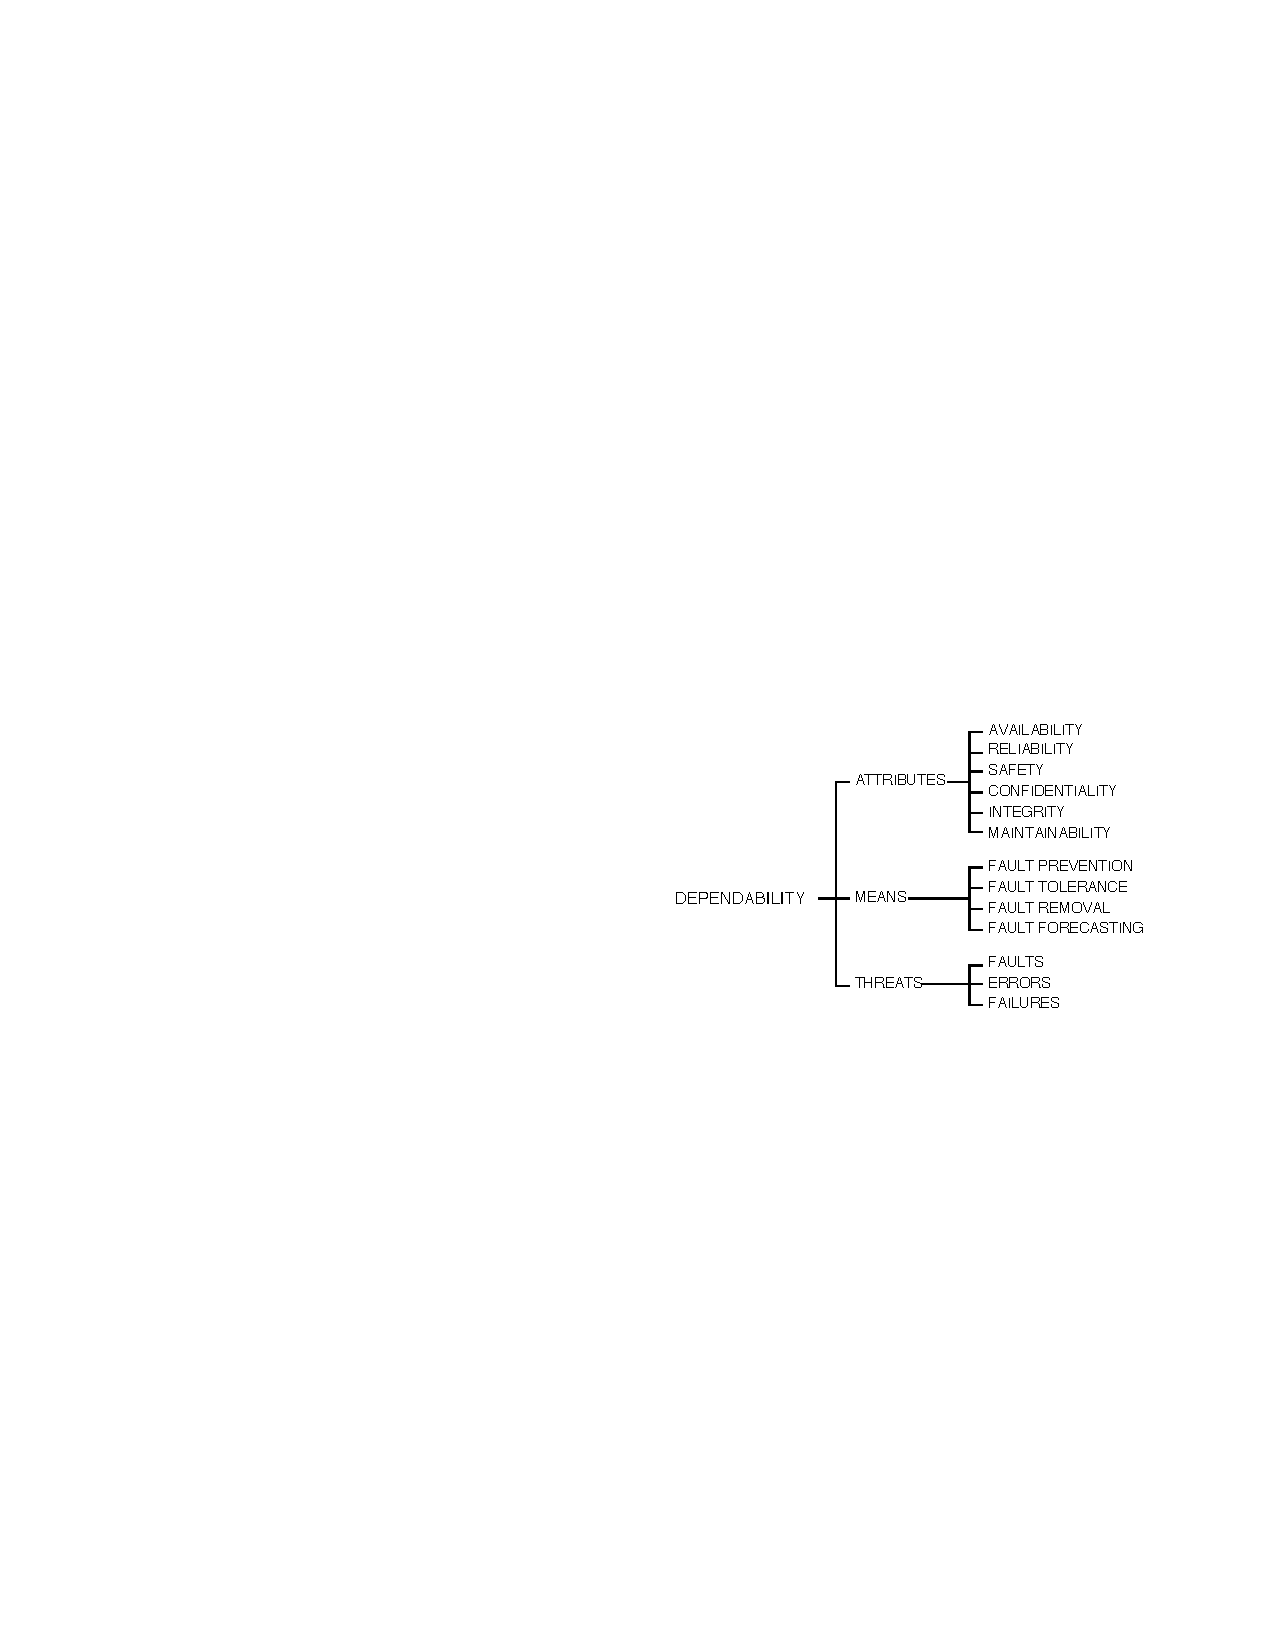
\includegraphics[width=0.8\columnwidth] {images/laprie.pdf}}
  \caption{The dependability tree by Laprie~\cite{Laprie2000}}
  \label{fig:laprie}
\end{figure}

% Goals of dependability reasoning:
%   - prediction of system failures
%   - comparison of competing designs: reason about how a change impacts dependability
%   - fullfil certification (not interesting to us)

\subsection{Dependability threats}
\label{subsec:dependability_threats}

The user has expectations over the service to be delivered by a system. These expectations may be formalized in a \emph{specification}. The delivered service can be split in two main categories: \textbf{correct} service and \textbf{incorrect} service (after Laprie~\cite{Laprie2004}). The specification may include both, even though it is more common for the specification to only include the expectations of correct service.

An example for a specification is a description of a service using the HTTP protocol~\cite{rfc2616}. The HTTP protocol specifies a request/response style message flow between a client and a server. The specification may include the location of the HTTP resources, how requests may be formed and which responses are to be expected. The specification may also include expectations for incorrect service. Each HTTP response message includes a numerical status code. If the server can not fulfill a request due to an error in itself or in its dependencies, it may use a status code equal to or higher than 500 to signify incorrect service to the client.

In the event of incorrect service being delivered, we call that a service failure, or short \textbf{failure}. The failure occurs at the moment when the user experiences incorrect service. There are different ways of how failures manifest themselves. We will reflect on some cases in \nref{ss:failure semantics}.

The reason for a failure to occur is the system being in an erroneous state, or short \textbf{error}. This means that the internal state of the system allowed a failure to occur. It is to be noted that an error is the state of the system and not an event. Only in the event of the user requesting the system's service does an error turn into a failure.

An example for an error is a server that has crashed. It is then in a state where it can not answer any client requests. The system can be in this state for a period of time, but a failure event only occurs in the moment when the client executes a request against the server.

A \textbf{fault} is the ``adjudged or hypothesized cause of an error''~\cite{Laprie1995}. Given that a fault is active, it is the cause of an error, thus there is an implication from fault to error. It is often hard to do that deduction the other way around, thus to identify the cause of an error as an exact fault. As engineers we may not be able to detect the faults themselves, but only the errors they have caused\footnote{For reference see section 3.3. in \cite{FundamentalsDepComputing}}. Therefore we use the qualifiers \emph{adjudged} and \emph{hypothesized} in the definition.

An example for a fault is a software bug which manifests itself as a single line of code and causes the server to crash when it is executed. When the software bug is in the software's codebase we call it a \emph{dormant} fault. As long as the line of code is not executed, the fault remains \emph{dormant}. It is activated the moment where the line of code is executed and then becomes an \emph{active} fault which subsequently puts the executed software into an erroneous state.

\begin{figure}[!h]
  \fbox{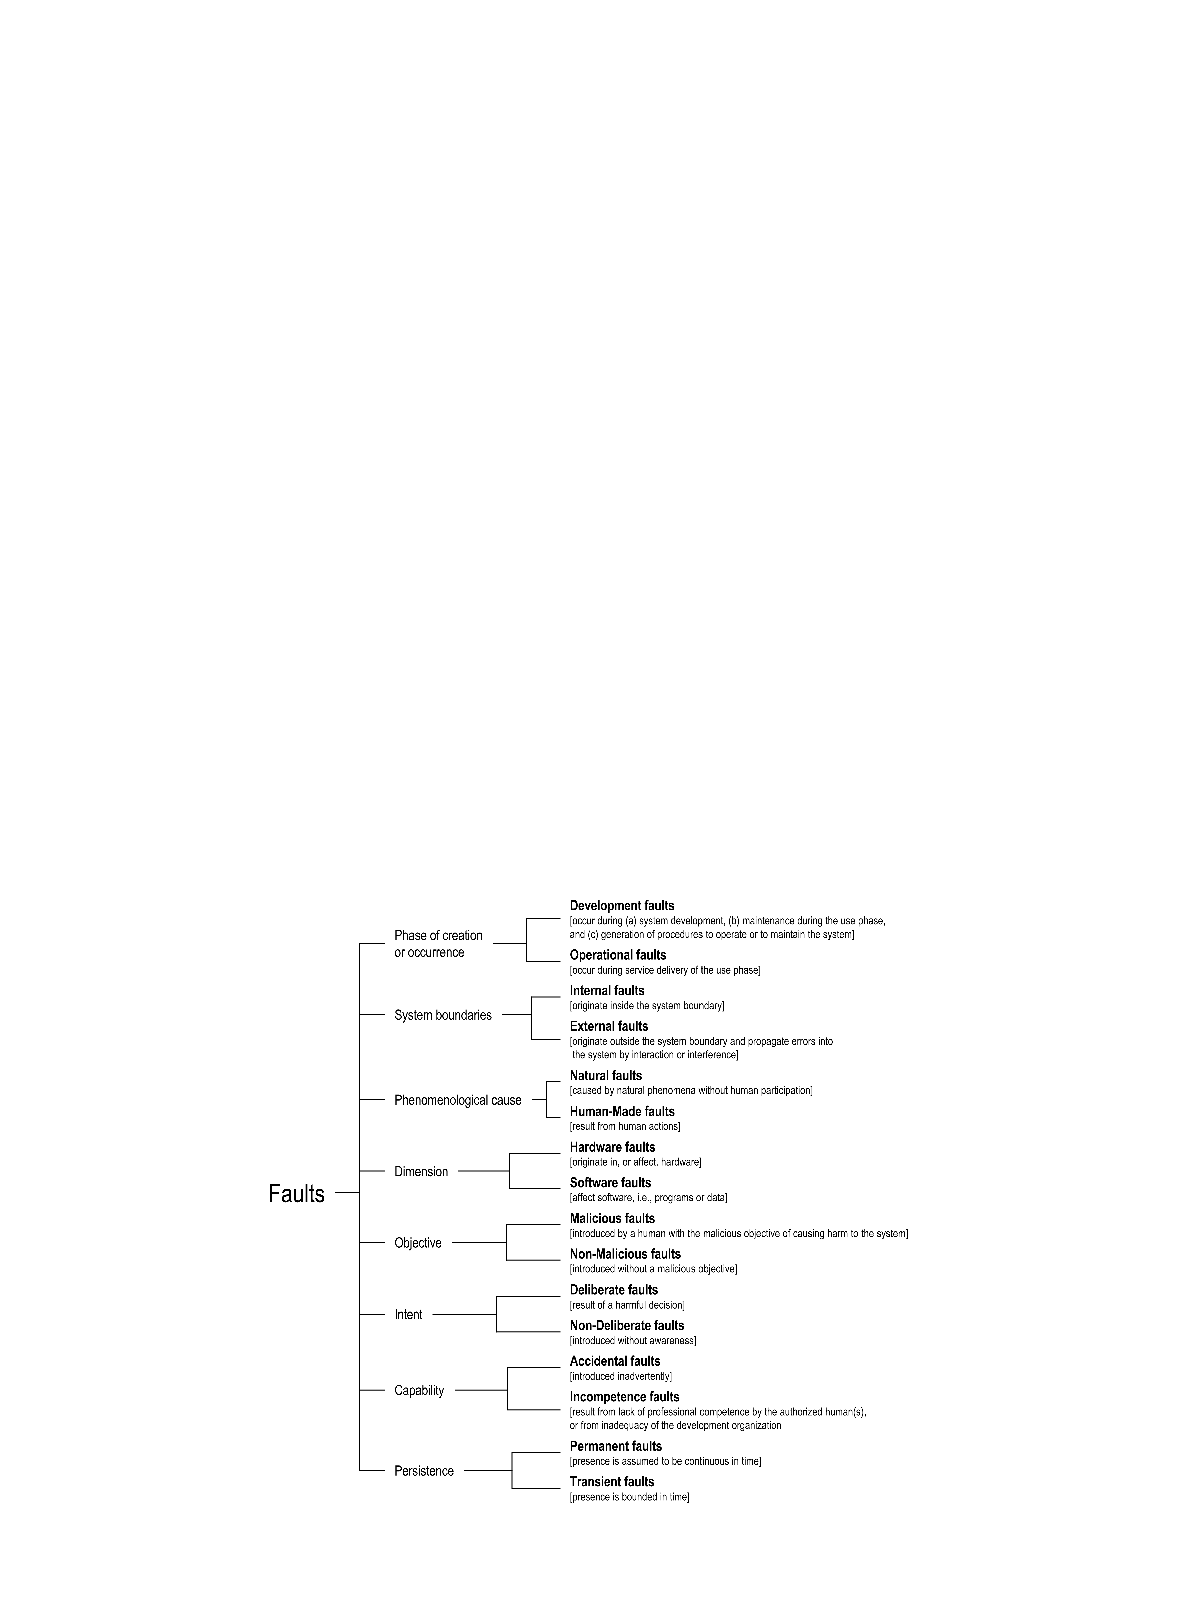
\includegraphics[width=\columnwidth] {images/faults.pdf}}
  \caption{The elementary fault classes by Laprie~\cite{Laprie2004}.}
  \label{fig:faults}
\end{figure}

Faults can be classified more precisely. Figure \ref{fig:faults} shows the elementary fault classes after Laprie. For this work, we are interested in classifying faults by \emph{system boundary}. A system boundary is defined by Laprie~\cite{Laprie2004} as ``the common frontier between the system and its environment''. The environment are all other systems that are not the system of interest. A system itself may contain other systems (usually called sub-systems or components). When classifying faults, we separate between \textbf{internal} and \textbf{external} faults.

An \emph{internal} fault originates within the system boundary. To illustrate this with an example we take a computer as a system. Internally, the computer consists of many components as sub-systems. The failure of one of the components (e.g. the memory) is a fault within the system, thus an \emph{internal} fault.

An \emph{external} fault originates from outside the system boundary. To illustrate, we again take the computer as an example. This time, we see the computer components CPU and memory as two separate systems. The CPUs correct service relies on the memory to work correctly. The failure of the memory may therefore be a fault to the CPU. Since the memory is not in the CPU, this is an \emph{external} fault to the CPU.

This hints to an interesting property, when looking at larger networks of systems that rely on each other: The failure of one system becomes the external fault of another system, which relies on it. We call this the \textbf{chain of dependability threats} (after the ``chain of threats'' by Laprie~\cite{Laprie2004}).

Figure~\ref{fig:depchain} visualizes the relation of fault-error-failure, as well as the chain of dependability threats. The arrows depict causation, from cause to effect. The boxes depict the system boundaries. \emph{System B} relies on \emph{System A}, therefore the failure of \emph{System A} may be seen as a fault in \emph{System B}.

\begin{figure}[!h]
  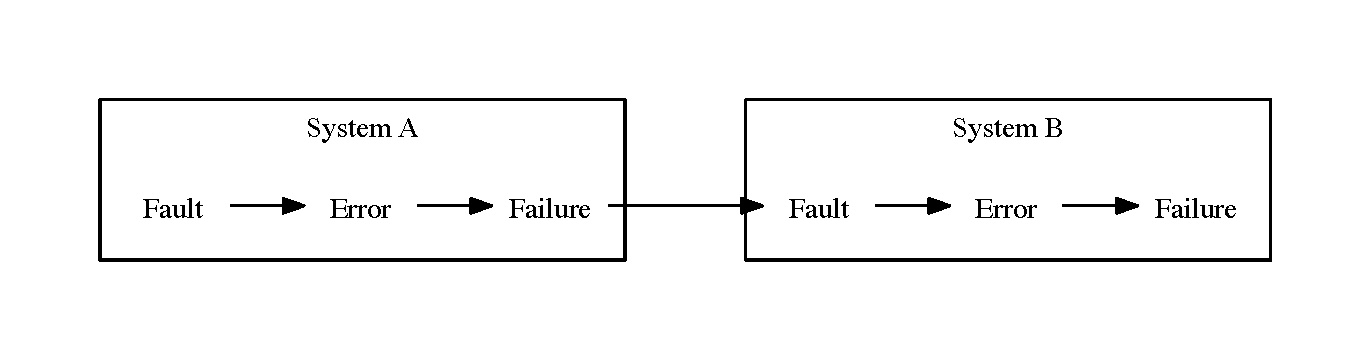
\includegraphics[width=\columnwidth] {images/chain-of-dep-threats.pdf}
  \caption{Chain of dependability threats}
  \label{fig:depchain}
\end{figure}

\subsection{Failure semantics}
\label{ss:failure semantics}

Failure semantics denote how a system and specifically its service to other systems behave in case of a fault (after Knight~\cite{FundamentalsDepComputing} section 3.8). They therefore set expectations for correct and incorrect service such that other systems may be able to guard against these.

One specific model for failure semantics was proposed by Cristian \cite{cristian}. His model is based on the notion of services (take input, execute operation, deliver output), servers who implement these services and a ``depends upon'' relation, in which the correctness of one server depends on the correctness of another server. The model then distinguishes between the following types of failures, notable within the ``depends upon'' relation:
\begin{tdescription}
  \item[Response failure] The response is incorrect. It could be in a wrong format or carry incorrect data.
  \item[Timing failure] The response happens outside of a specified time interval
  \item[Omission failure] No response is ever delivered for a request
  \item[Crash failure] After an initial omission failure all subsequent requests exhibit omission failures as well until the system is restarted
\end{tdescription}

We will build on this model later, when we propose our algorithm for constructing fault trees in \autoref{chapter:fault_trees} and explain our concrete assumptions regarding the failure semantics of the systems.

\subsection{Dependability means}
\label{subsec:dep_means}

Dependability means are ways to limit the impact of dependability threats on the dependability of a system. Following the list of means from \autoref{fig:laprie}, they include fault prevention, fault tolerance, fault removal and fault forecasting. All means focus on faults and ways to mitigate them, in order to not have them propagate to failures.

Dependability means are not in the scope of this work. For more information on this topic we recommend the work of Knight \cite{FundamentalsDepComputing}.

\subsection{Dependability attributes}
\label{sec:theory_dep_attrs}

The attributes of dependability define the different aspects, as to which the dependability of a system can be evaluated. The dependability means are there to assure these attributes against the dependability threats. In previous \autoref{fig:laprie} six attributes are mentioned. In the scope of this work we are only interested in \emph{reliability} and \emph{availability}:

\paragraph{Reliability} is defined by Laprie \cite{Laprie2004} as the ``continuity of correct service''. A more concrete definition is delivered by Knight \cite{FundamentalsDepComputing} as ``R(t) = probability that the system will operate correctly in a specified operating environment up until time t''. We assume that at the time t=0, the system was operating correctly. R(t) then denotes the probability that in the interval [0,t] the system has not suffered a failure. An underlying assumption of this reliability definition is that the system is not repairable: given that a failure occurred, the system stays in an incorrect state and may never return into a functioning correct state again.

%In the context of this work, we are concerned with software. One of the properties of software is, that it may recover from failures. This can be achieved by implementing fault tolerance mechanisms. To model this property, availability may be used.

\paragraph{Availability} is defined by Laprie \cite{Laprie2004} and Goloubeva \cite{Goloubeva2006} as ``readiness for correct service''. In contrast to reliability, availability allows for systems to be repairable after a failure occurred. Thus, a system might fail, be repaired and then deliver correct service again. During the time of repair we assume the system to deliver incorrect service.

Please note that in later \autoref{subsec:historical_availability_theory} we introduce more theoretical background, which is utilized when calculating failure probabilities from historical availability.

\subsection{Fault tree analysis}
\label{subsec:theory_faulttree}

\subsubsection{Introduction}

When we talk about dependability in systems, we eventually aim to prevent failures. For that we have to analyze the system. To do this in a structured way, many methods exist. Three notable are \emph{Failure modes, effects and criticality analysis (FMECA)}~\cite{FMEA}, \emph{Reliability block diagrams} (\cite{SysReliabilityTheory} section 3.10.), and fault tree analysis, which we will treat further in this section. All methods share the common assumption that faults happen. We may then separate faults into two categories: \emph{anticipated} faults and \emph{unanticipated} faults (\cite{SysReliabilityTheory} section 4.1). Against anticipated faults we are able to deploy dependability means. But against unanticipated faults we can by definition not defend, thus these are the most likely to propagate to failures. Therefore, one of the goals of structured methods for dependability analysis is identifying these faults as comprehensively as possible, so that they can be anticipated.

Next, we will introduce fault tree analysis further. It originated in the Bell Telephone Laboratories in 1962 for evaluating systems of the \emph{Minuteman} missile program~\cite{ericson1999fault}. It also found application in nuclear power stations~\cite{NuclearFT} and aerospace missions~\cite{NasaFT}.

\subsubsection{Definition}

A \textbf{fault tree} is defined by Rausand et al \cite{SysReliabilityTheory} as a ``logic diagram that displays the interrelationships between a potential critical event [...] in a system and the causes for this event''. Fault tree analysis is the process of constructing such a fault tree. A fault tree may be qualitative or quantitative, which we both will describe next.

\subsubsection{Qualitative fault trees}

A fault tree analysis is started by defining the system failure to investigate. We call that the \emph{TOP event} of the fault tree. From that event, all events that might contribute to its occurrence are identified as new events. They are connected to the \emph{TOP event} via the \emph{logic gates} \emph{AND-gate} or \emph{OR-gate}. This process is continued for all new events recursively, until a sufficient level of detail is reached. Thus, we acknowledge that any event can likely be seen as consisting of a more detailed fault tree, but we make the design decision for the fault tree to stop investigating this greater detail. Since the analysis method is from top down, we call it ``deductive''. The leafs of the resulting tree are called \emph{basic events}. If an event is neither \emph{basic} nor \emph{TOP} event, it is called \emph{intermediate event}.

Table \ref{tab:faulttreeelements} shows all the fault tree elements with their graphical symbols from the Fuzzed Editor~\cite{fuzzed}\footnote{All fault trees in this work were generated using the Fuzzed Editor~\cite{fuzzed} and therefore share the graphical symbols introduced here}. More elements for fault trees exist (e.g. explained in \cite{NuclearFT} and \cite{NasaFT}), but for our case the introduced elements are sufficient.

\begin{table}[!h]
  \centering
  \caption{Fault tree elements}
  \label{tab:faulttreeelements}
  \small
  \begin{tabularx}{\linewidth}{ |l|m{1.35cm}|X| }
    \hline
    Name & Symbol & Description \\
    \hline
    TOP event & 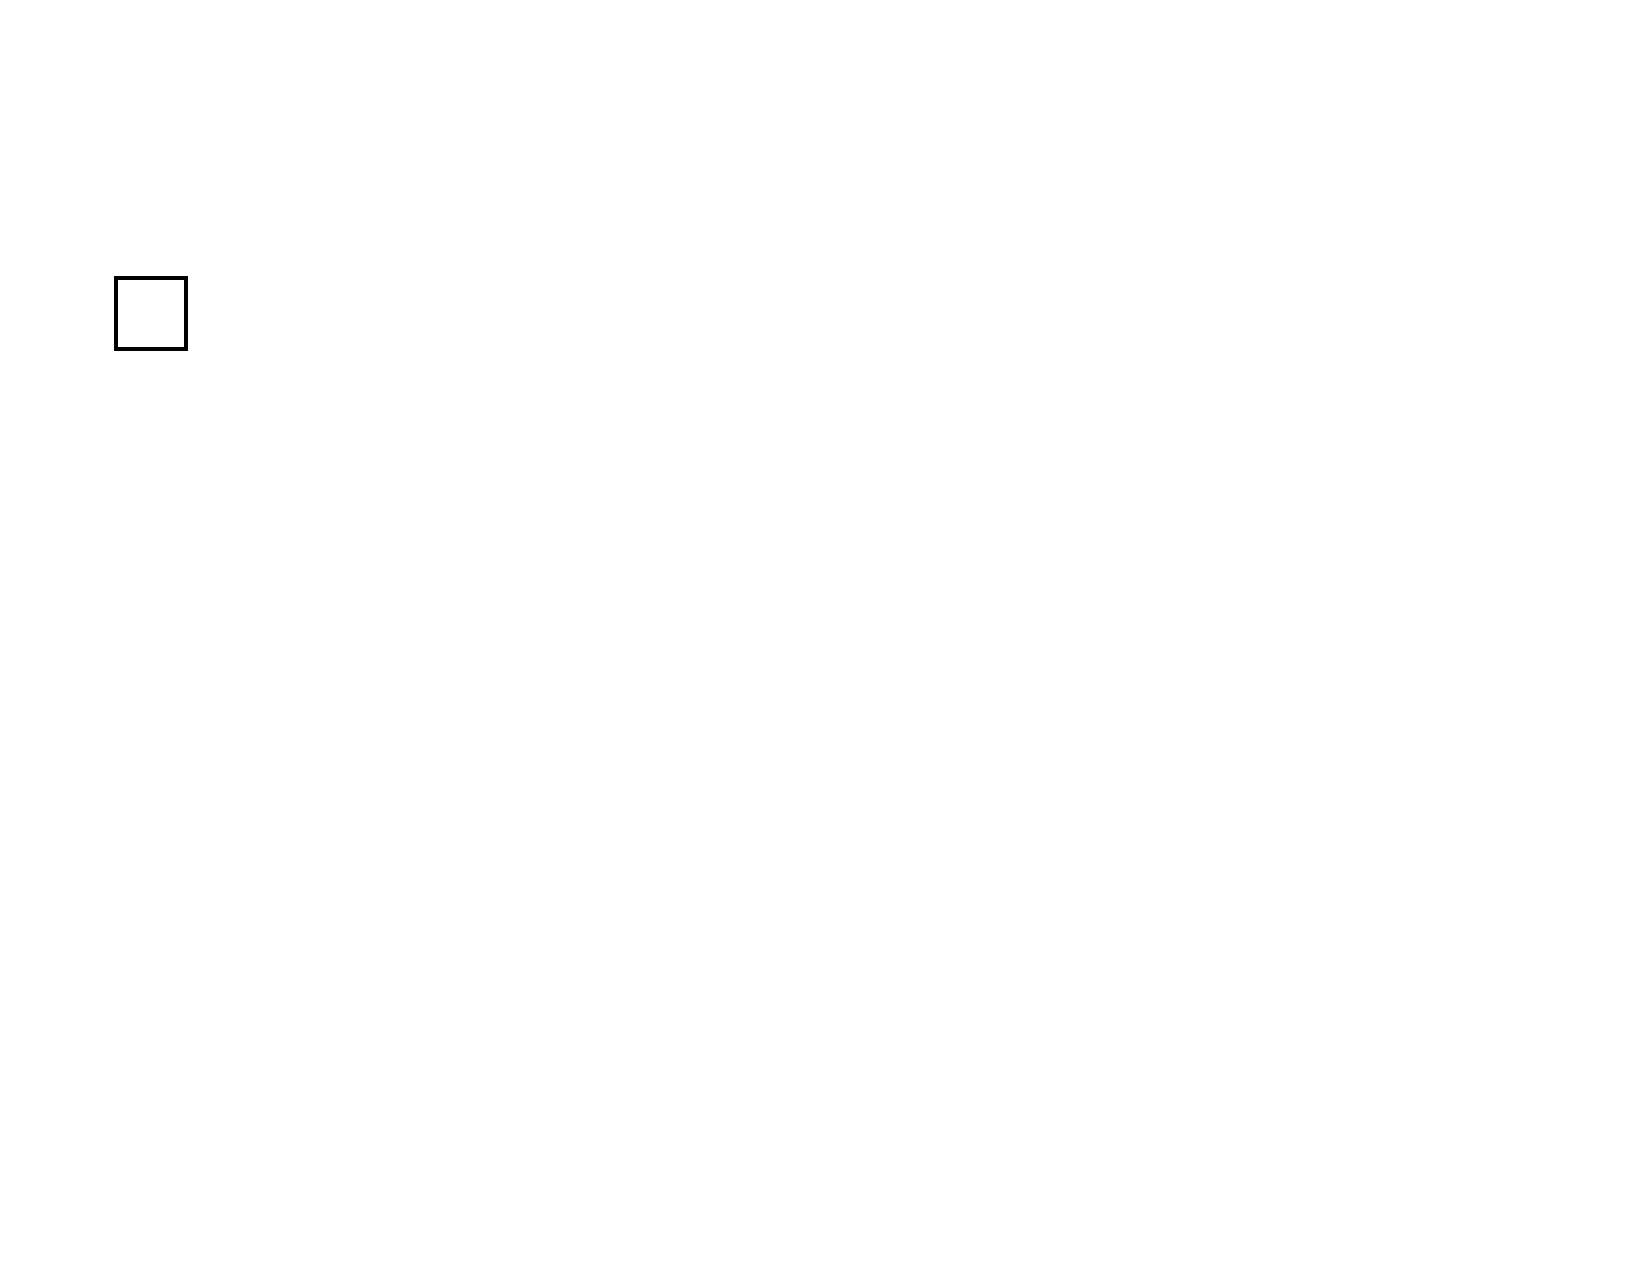
\includegraphics[keepaspectratio=true,scale=0.8] {images/fault-tree-top-event.pdf} & The TOP event, is the event whose causes are investigated with the fault tree. A fault tree may only have one TOP event. \\
    \hline
    AND-gate & 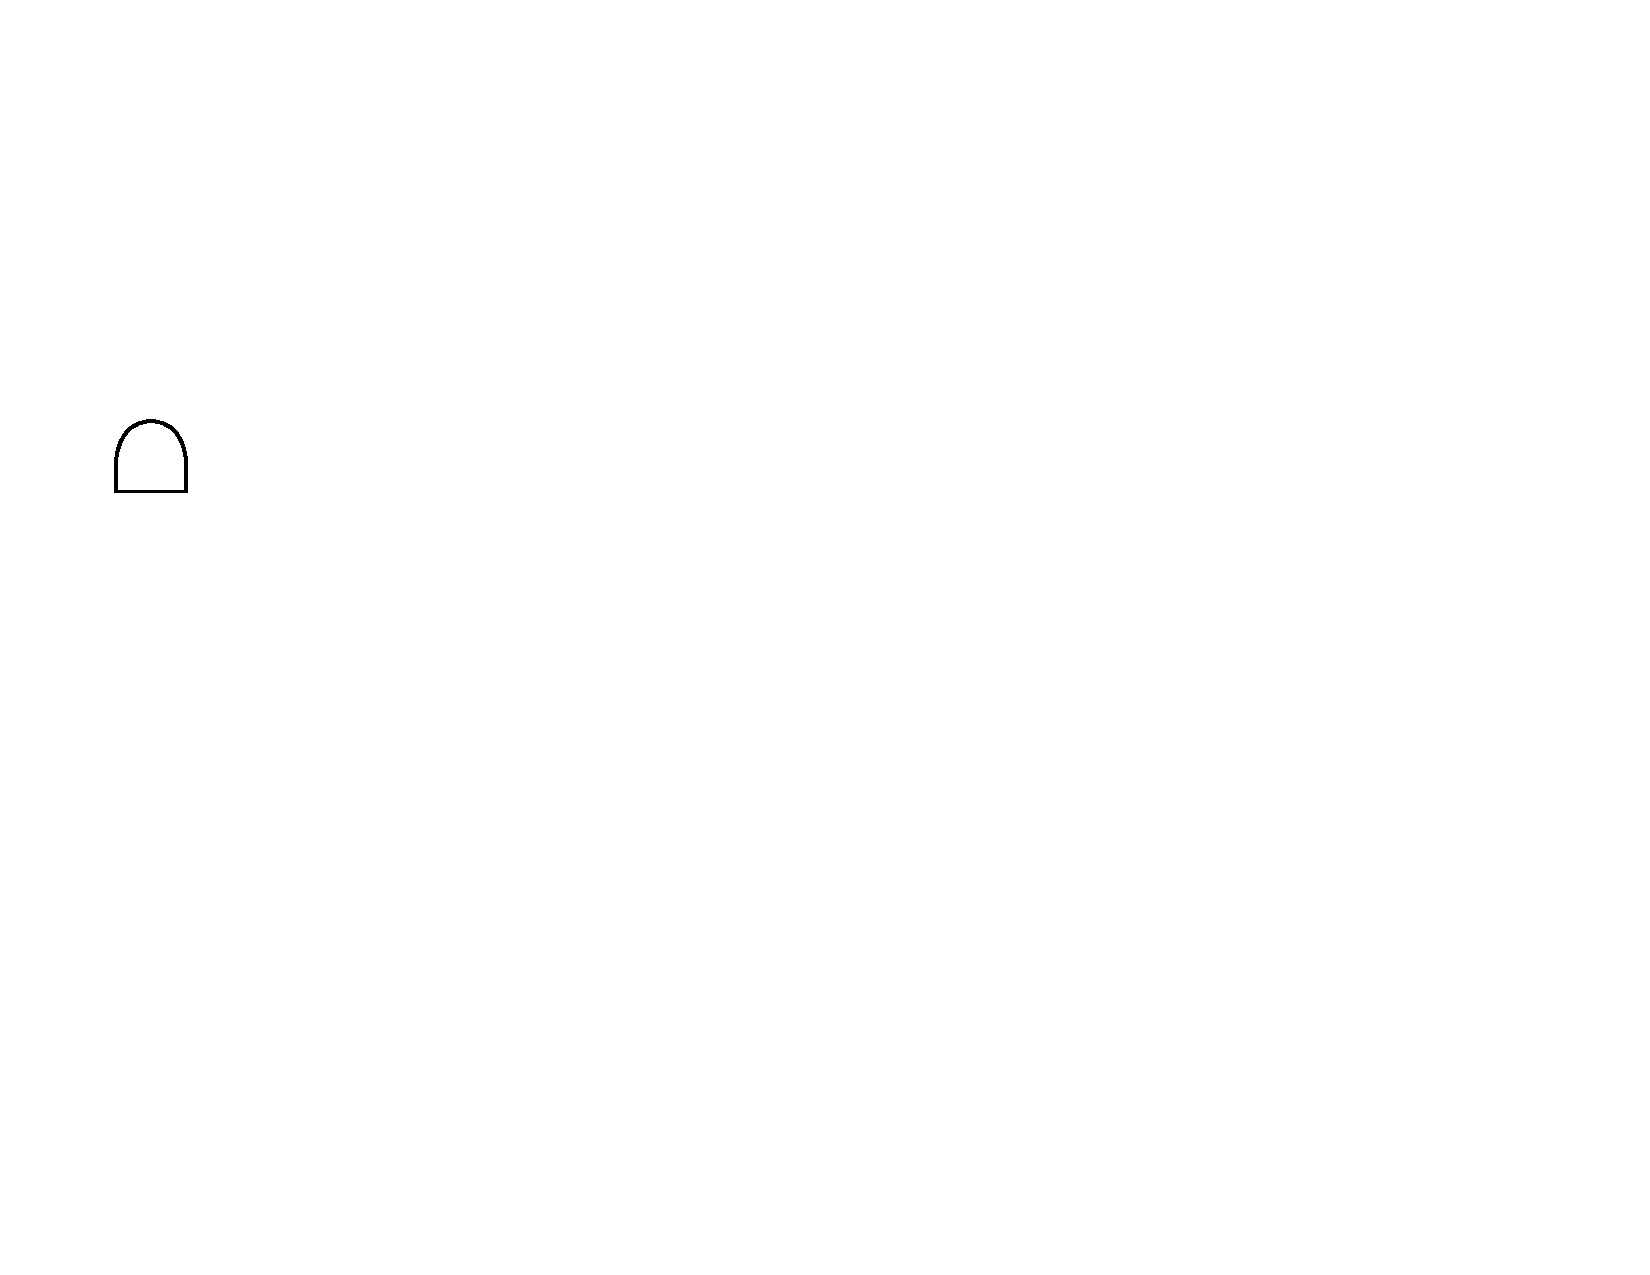
\includegraphics[keepaspectratio=true,scale=0.8] {images/fault-tree-and-gate.pdf} & An AND-gate connects many input events with one output event. The output event occurs only when all input events occur. \\
    \hline
    OR-gate & 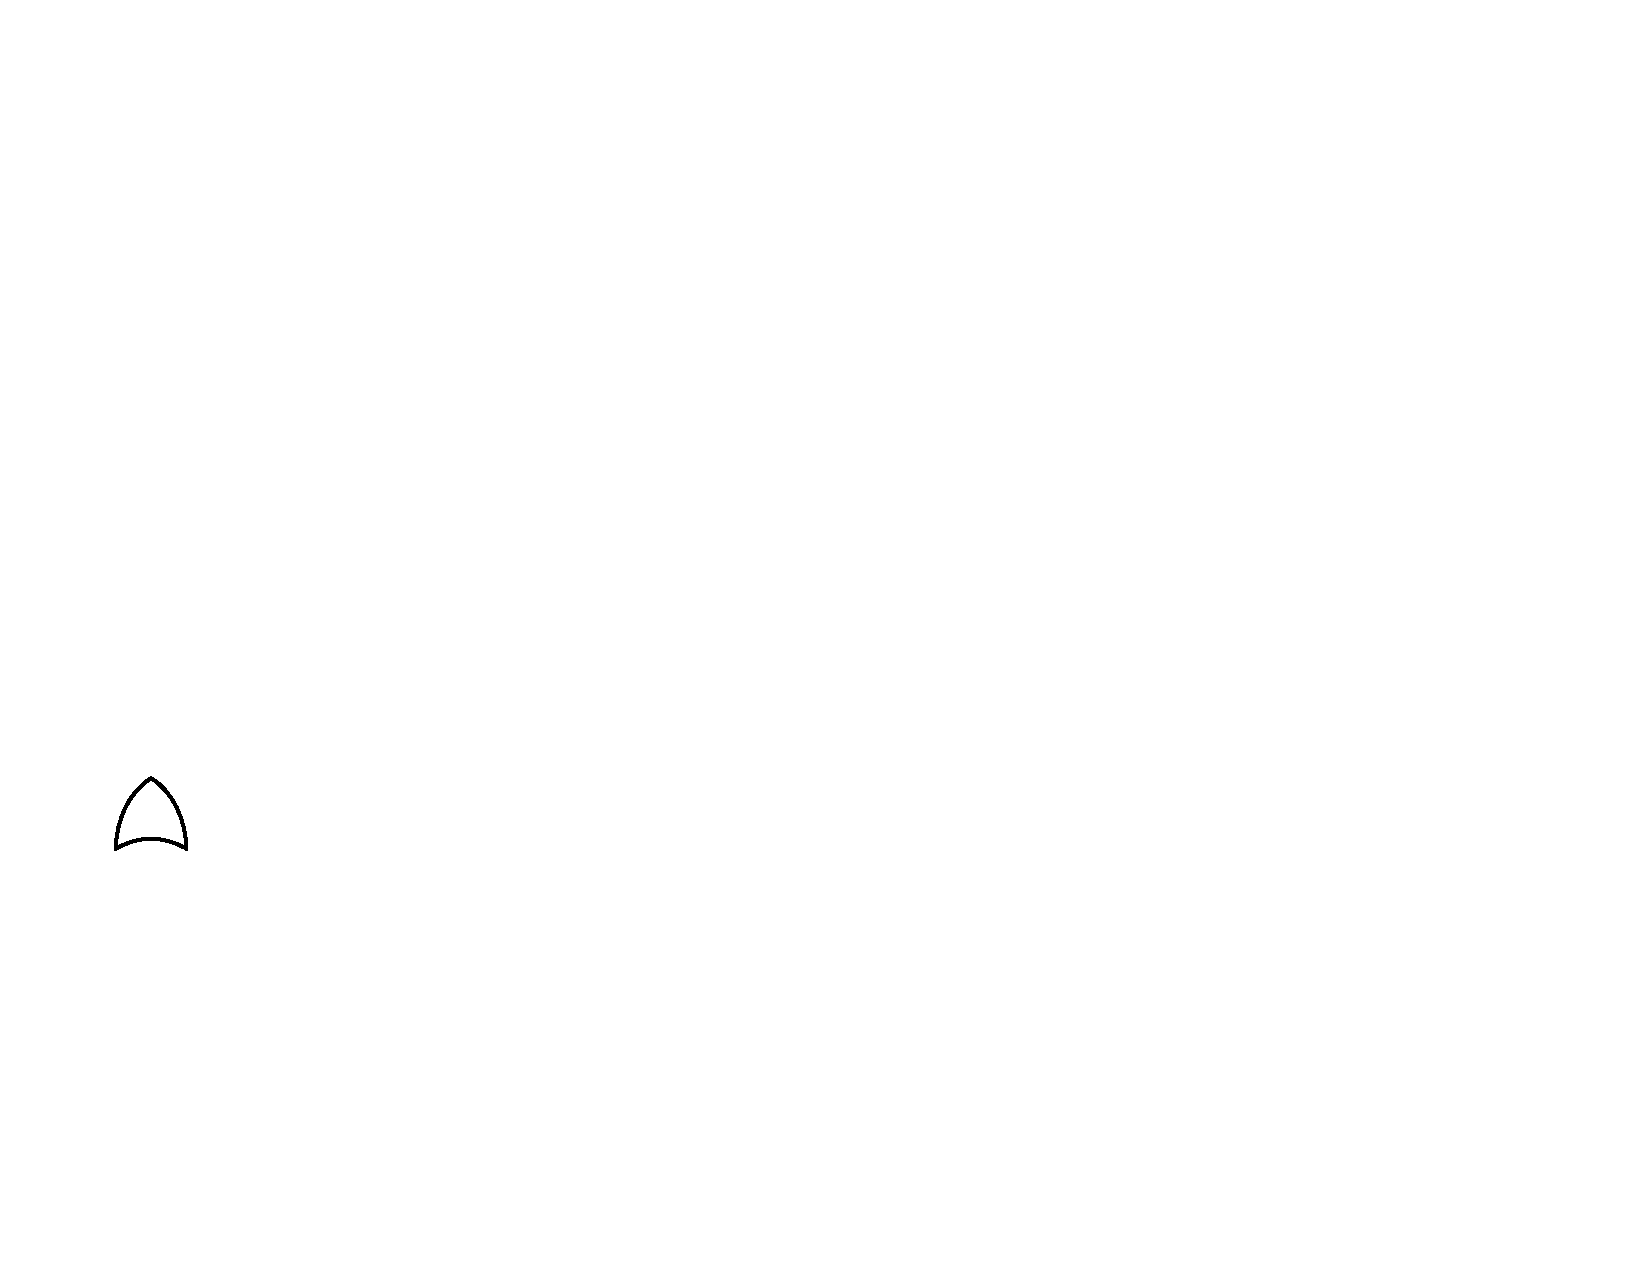
\includegraphics[keepaspectratio=true,scale=0.8] {images/fault-tree-or-gate.pdf} & An OR-gate connects many input events with one output event. The output event occurs if any of the input events occurs. \\
    \hline
    Intermediate event & 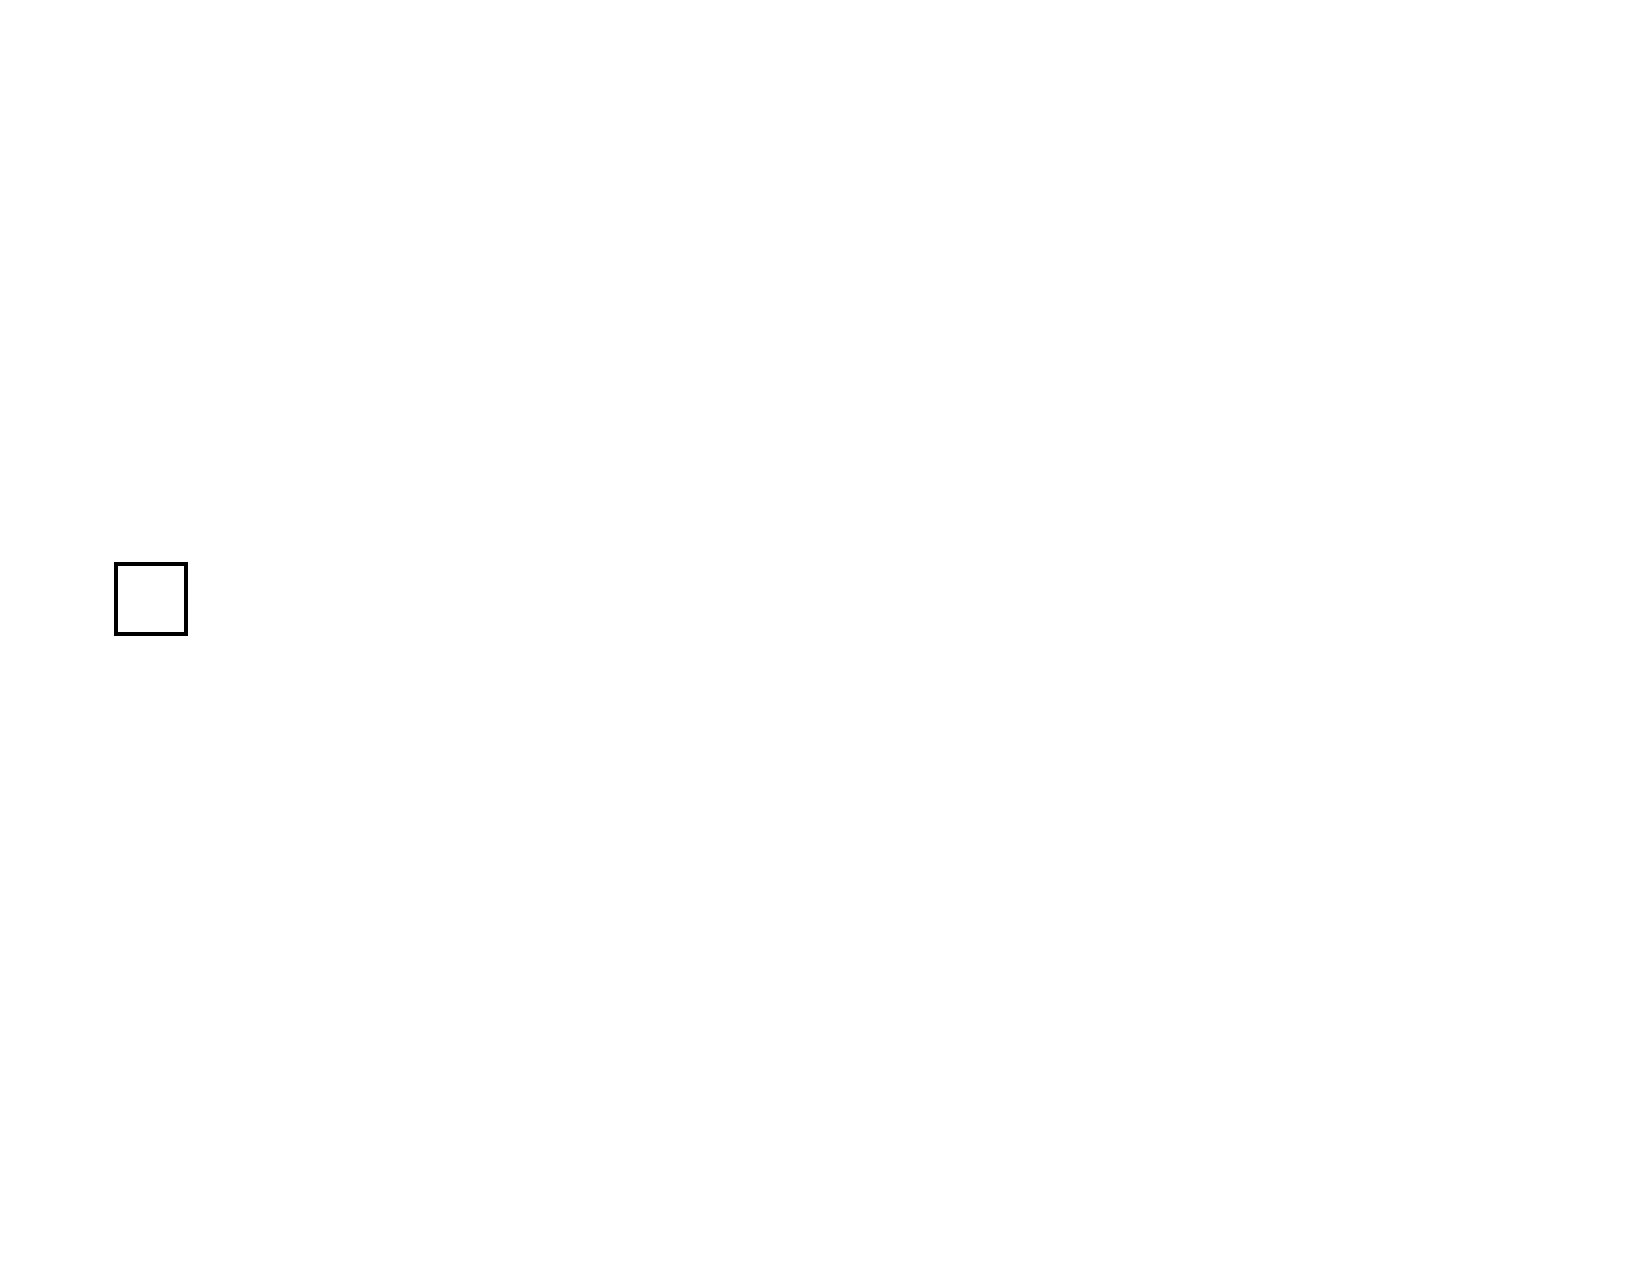
\includegraphics[keepaspectratio=true,scale=0.8] {images/fault-tree-intermediate-event.pdf} & An intermediate event may be used as event between logic gates.\\
    \hline
    Basic event & 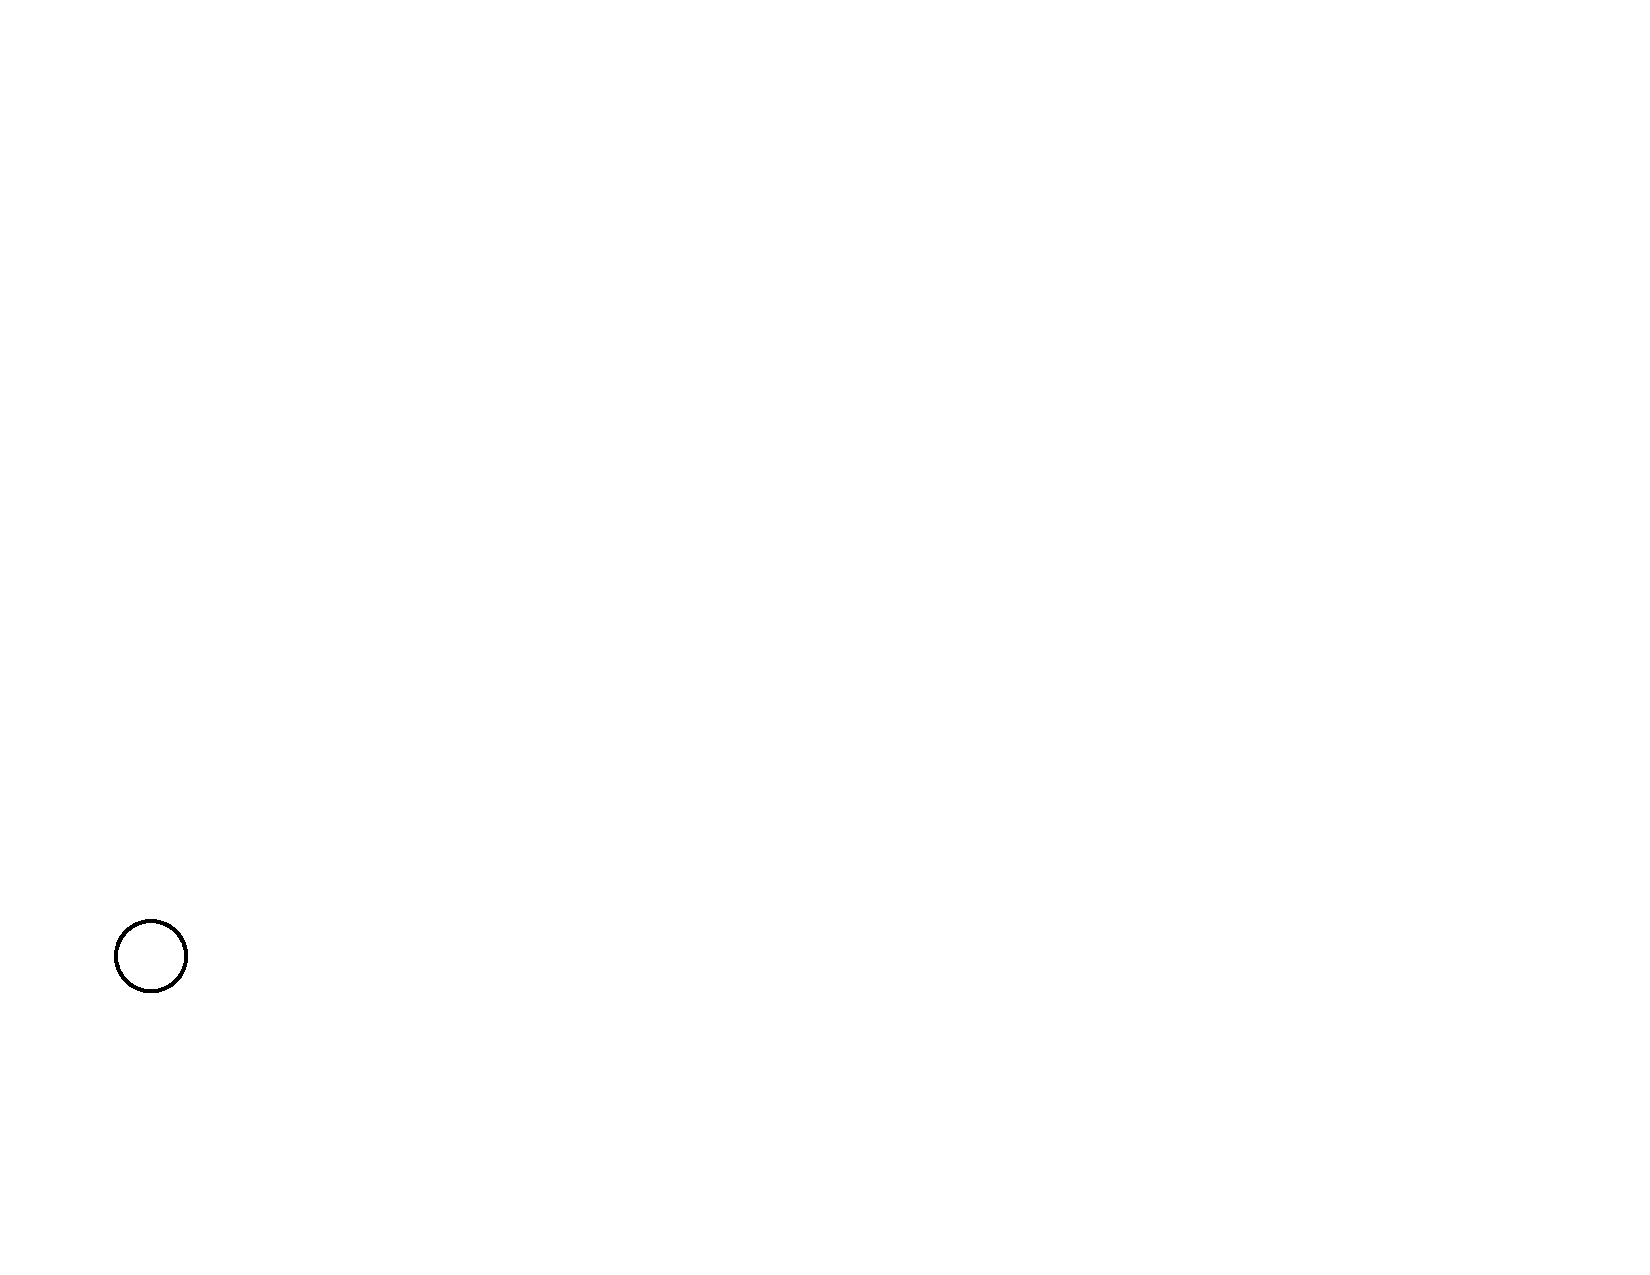
\includegraphics[keepaspectratio=true,scale=0.8] {images/fault-tree-basic-event.pdf} & A basic event represents the occurrence of a specific failure event. A basic event may have a failure probability assigned.\\
    \hline
  \end{tabularx}
\end{table}

Figure~\ref{fig:fault-tree-example-qualitative} shows an example qualitative fault tree. It can be seen that there is one TOP event. ``Intermediate Event'' occurs if either ``Basic Event 2'' or ``Basic Event 3'' or both occur. ``TOP event'' occurs if ``Basic Event 1'' and ``Intermediate Event'' occur.

\begin{figure}[!h]
  \centering
  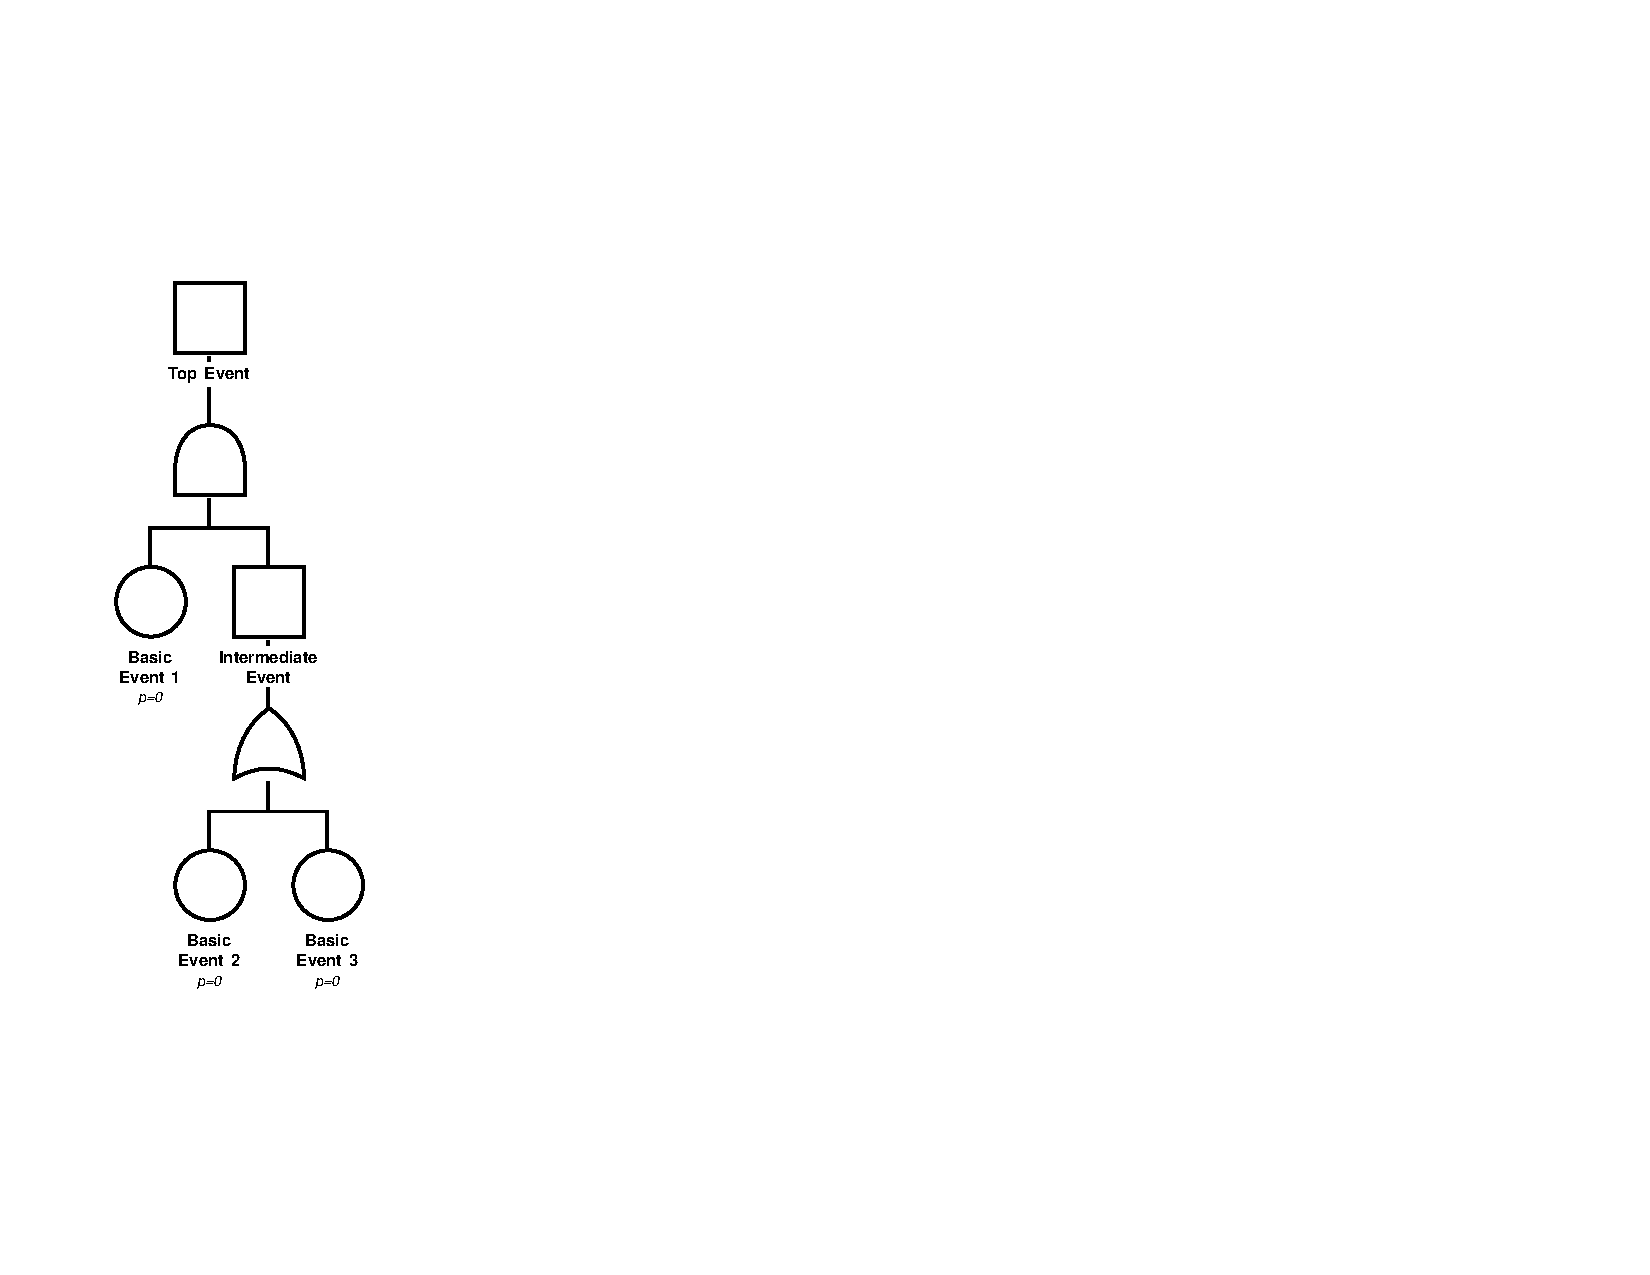
\includegraphics[width=0.25\columnwidth] {images/fault-tree-example-qualitative.pdf}
  \caption{Example qualitative fault tree}
  \label{fig:fault-tree-example-qualitative}
\end{figure}

When a qualitative fault tree exists, it may be analyzed for possible combinations of basic events that result in the TOP event (called ``cut sets'', for example explained by Rausand et al~\cite{SysReliabilityTheory} section 3.6.4.). For example this analysis then allows for the identification of single point of failures in the system.

Another value of fault trees is running the fault tree analysis itself. The analysis process involves gathering experts and addressing the problem of dependability of a system from many different viewpoints. During the process, many problems and maybe even their respective solutions may become apparent. The resulting fault tree may then be used as basis for discussion, for example to communicate the current state of the system or discuss potential changes.

\subsubsection{Quantitative fault trees}

Quantitative fault trees allow for calculating the probability of the TOP event based on the probabilities of the basic events. A quantitative fault tree analysis may use the same fault tree structure as the qualitative fault tree. Next, we will explain how such a calculation may be carried out. We base the following calculations after Limnios \cite{FaulTreesLimnios} chapter 5.

We operate under the following assumptions:
\begin{titemize}
  \item Every basic event may exist in the fault tree only once. Repeated basic events are not allowed.
  \item The basic events are independent events.
  \item The calculations are done for repairable systems.
\end{titemize}

Furthermore we assume that all basic events have a failure probability. We may now calculate the probability per logic gate: We assume A and B to be the logic gate inputs with Pr(A) and Pr(B) being their respective failure probabilities. E is the logic gate output, with the resulting failure probability Pr(E).

Equation for an AND-gate:
\[ \begin{array}{lclcl}
E & = & A \cap B & & \\
Pr(E) & = & Pr(A \cap B) & = & Pr(A) * Pr(B)
\end{array} \]

Equation for an OR-gate:
\[ \begin{array}{lclll}
E & = & A \cup B & & \\
Pr(E) & = & Pr(A \cup B) & = & Pr(A) + Pr(B) - Pr(A) * Pr(B)
\end{array} \]

Both equations may be extended for more than two inputs. To calculate the TOP event probability, we may use the ``recursive inclusion-exclusion method''~(after Limnios~\cite{FaulTreesLimnios} section 5.5.1): We start at the TOP event and resolve the immediate logic gate. We then recursively resolve all input events after the same method. Following is the equation for earlier example fault tree~\ref{fig:fault-tree-example-qualitative}:

\[ \begin{array}{lcl}
Pr(TOP Event) & = & Pr(Basic Event 1 \cap Intermediate Event) \\
 & = & Pr(Basic Event 1) * Pr(Intermediate Event) \\
 & = & Pr(Basic Event 1) * ( Pr(Basic Event 2 \cup Basic Event 3)) \\
 & = & Pr(Basic Event 1) * ( Pr(Basic Event 2) + Pr(Basic Event 3) - \\
 & & Pr(Basic Event 2) * Pr(Basic Event 3))
\end{array} \]

As we can see, the resulting equation only has probability operators and therefore the probability of the TOP event is resolvable, given that each basic event has a probability assigned.

The major value we see in creating quantitative fault trees is for comparing changes to basic event probabilities and respective impact on the TOP event probability.
